\subsubsection{Prepare FFC cable}
To use FFC breakout board for debugging, FFC cables with ground shielding should
be purchased.

If normal FFC cables (it seems that, at least in the U.S., it is harder to find
properly-shielded FFC cables) are purchased, an additional manual modification
needs to be done on the optical mezzanine side of the cable connector:
A insulation tape (possibly Kapton tape) should be applied on the lower 1/4 of
the connector, so that the shielding pins on the optical mezzanine are masked
(ineffective).
See \autoref{fig:ffc_cable} for FFC breakout cable with modification.

\begin{figure}[!ht]
    \centering
    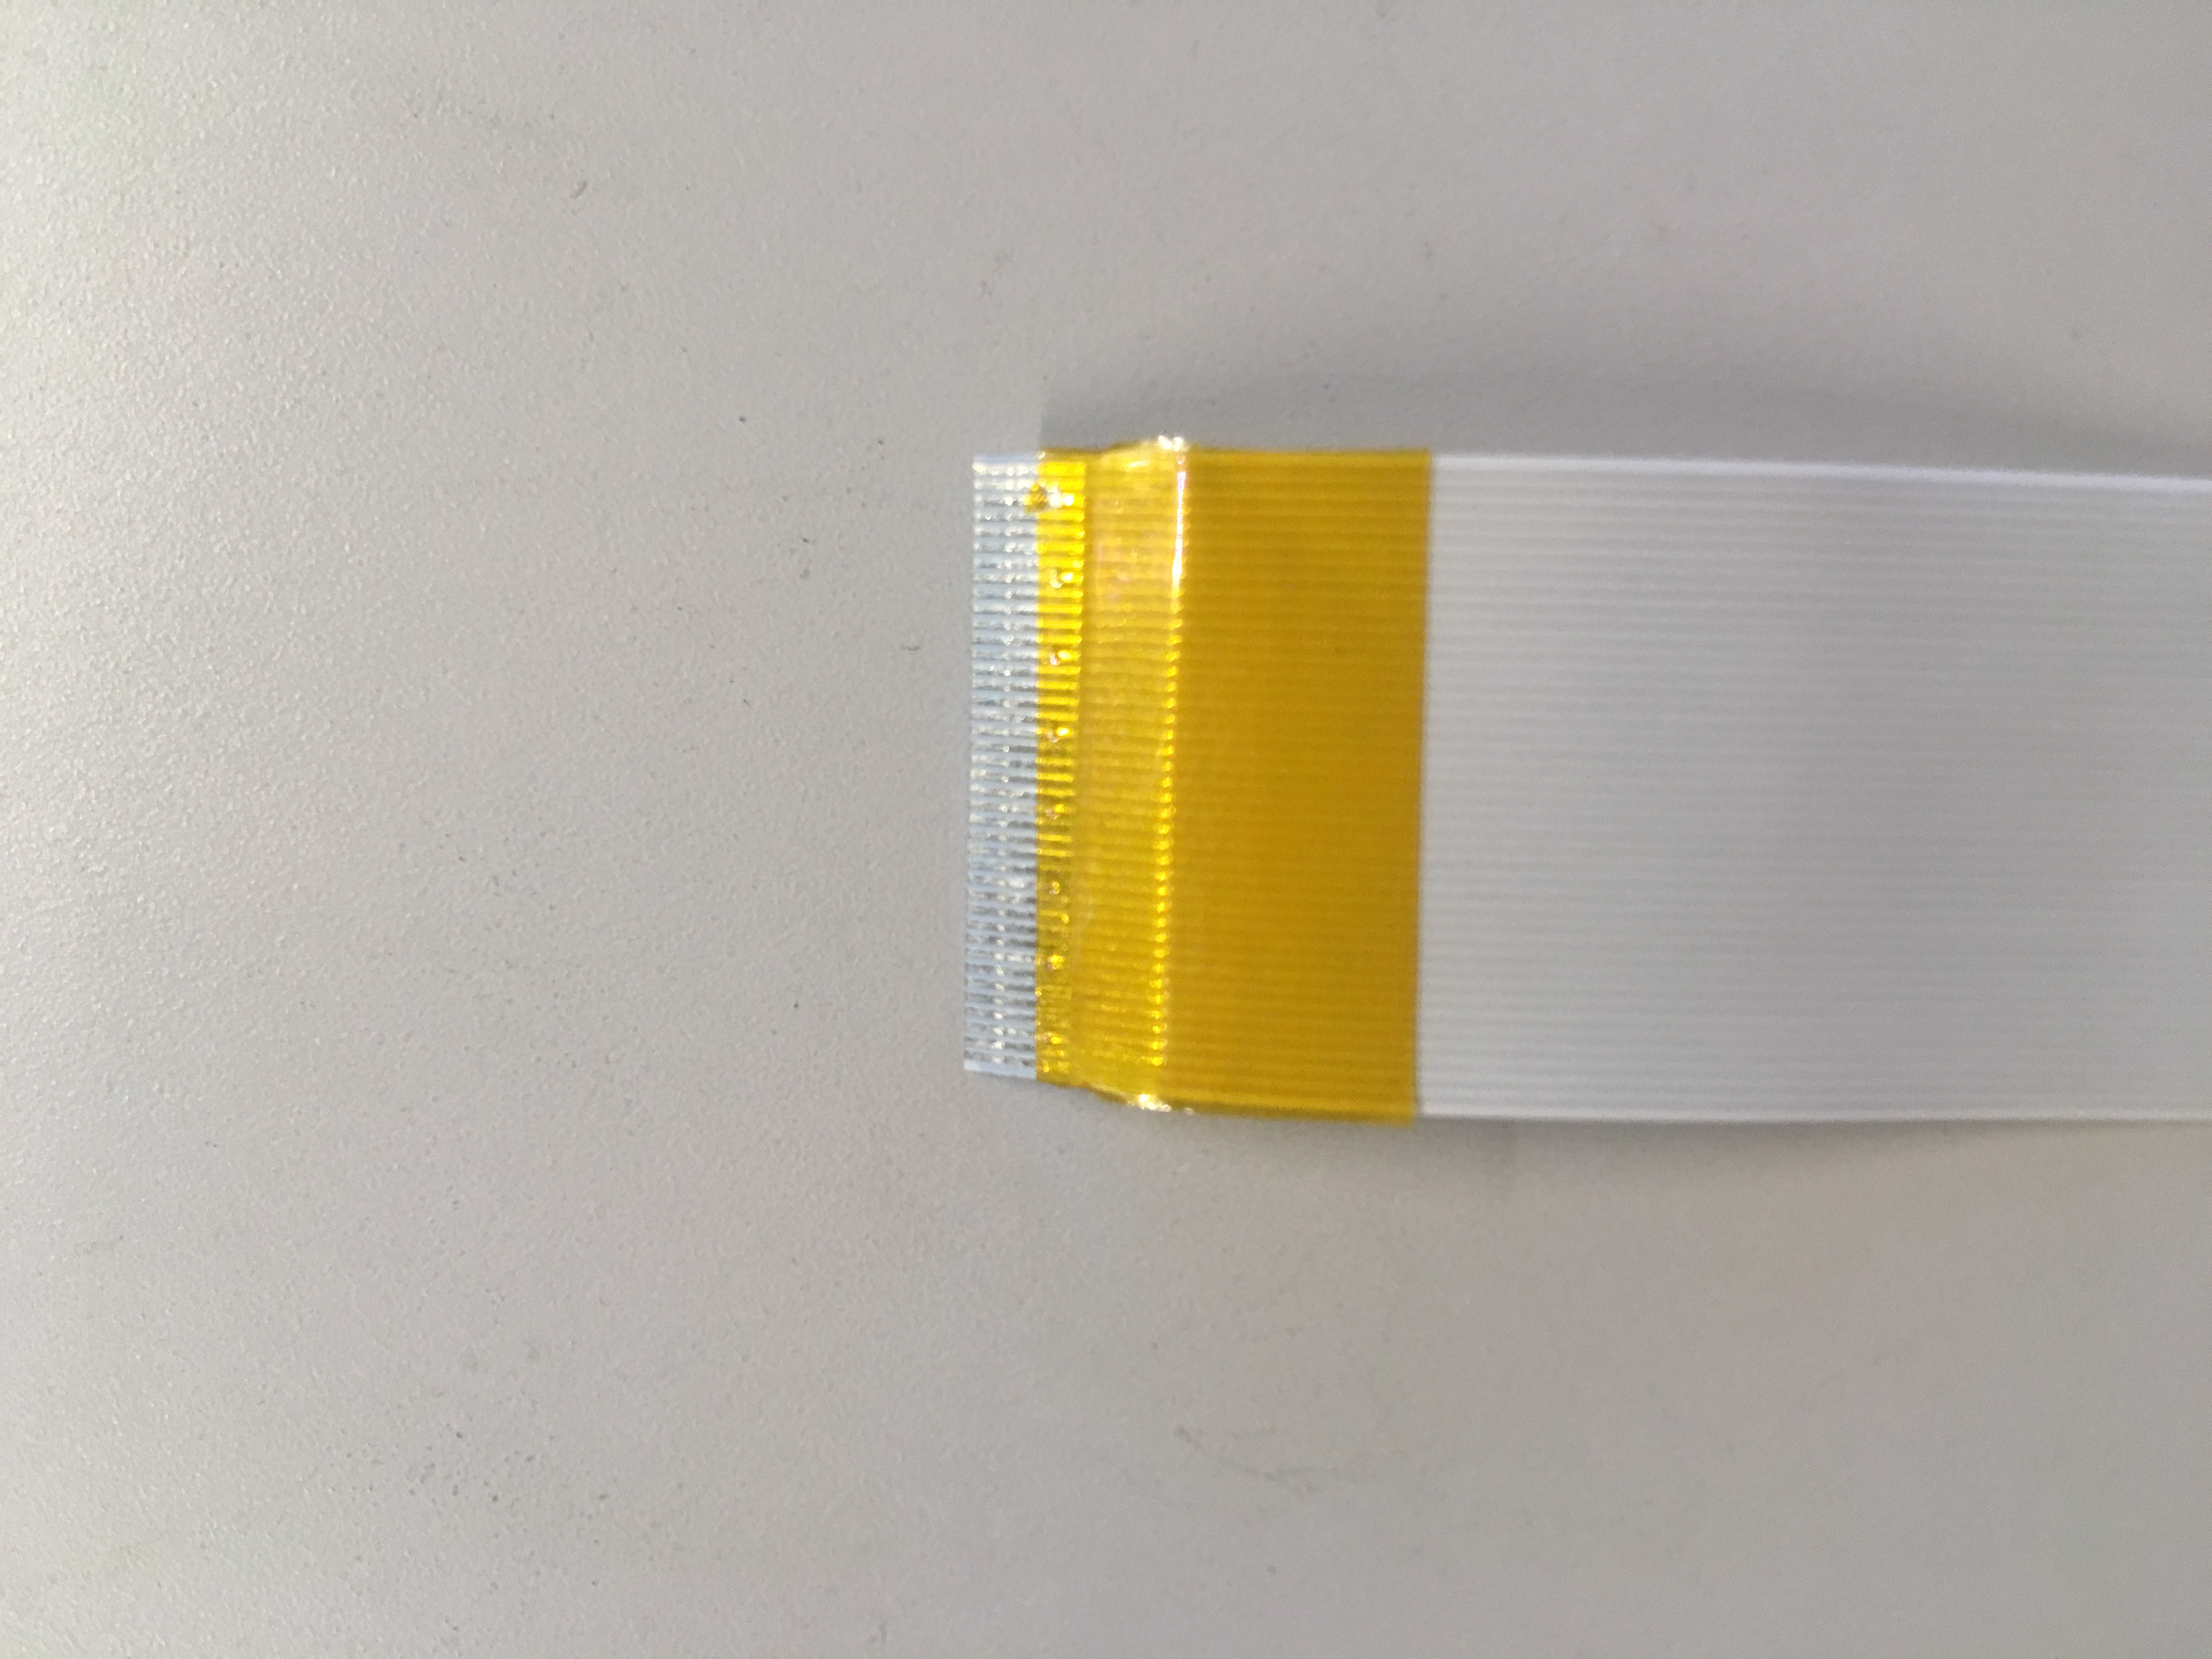
\includegraphics[width=0.9\linewidth]{res/ffc_breakout_cable_with_tape.jpg}
    \caption{FFC breakout cable with modification.}
    \label{fig:ffc_cable}
\end{figure}

\begin{leftbar}
    Note that after prolonged use, the metal contact pin may penetrate the
    Kapton tape on the FFC cable connector, rendering the trick shown in
    \autoref{fig:ffc_cable} ineffective.

    To fix the problem, redo the track;
    alternatively, trim the FFC cable connector to make it shorter---this should
    be a more permanent solution.
\end{leftbar}
